\topic{Functions (maps)}{Functions (maps)}
\begin{definition}
    \textbf{(Function).} Let $X$ and $Y$ be two non-empty sets. The \textbf{function}, or \textbf{map}, from $X$ to $Y$ is a subset $f$ of $X\times Y$ such that for each $x\in X$ that appears as part of a pair in $f$, there is one, and only one $y\in Y$ such that $\left( x, y \right)\in f$, and we write $f:X\to Y$.
\end{definition}
\begin{example}[An example of a function would be]
    \begin{align}
        f:\R&\to\R \quad\quad\quad\quad\quad f = \{( x, x^2 + 1)\tq x\in\R \}\subset\R\times\R = \R^2 \\ 
        x&\to x^2 + 1
    \end{align}
\end{example}
\begin{example}[A typical non-example of a function would be]
    \begin{equation}
        h:=\{( x,\ \pm \sqrt{x})\tq x\in\R \}\subset\R\times\R = \R^2 
    \end{equation}
    \begin{itemize}
        \item If $x < 0$ then $\pm\sqrt{x} \notin\R $.
        \item We would have two inputs for the very same input value: 
            \begin{equation}
                (2, \sqrt{2} )\in h,\ ( 2, -\sqrt{2})\in h
            \end{equation}
    \end{itemize}
\end{example}
\begin{definition}
    Let $f:X\to Y$ and let $g:X\to Y$ be two functions. We say that $f = g$ if $\forall x\in X,\ f\left( x \right) = g\left( x \right)$.
\end{definition}

\subsection{Domain, codomain and range of a function}
\begin{definition}
    Let $f:X\to Y$ be a function. Then, 
    \begin{itemize}
        \item $X$ is the \textbf{domain} of the function: the set containing all the input values of the function. Since a function is defined on its entire domain, its domain coincides with its domain of definition.
        \item $Y$ is the \textbf{codomain} of the function: the set containing all of the output values of the function.
        \item The \textbf{range} of the function is the subset of $Y$:
            \begin{equation}
                \textrm{Range }:=\{y\in Y\tq \exists\ x\in X \textrm{ with } f\left( x \right) = y\} 
            \end{equation}
    \end{itemize}

    %\begin{itemize}
    %    \item $A$ is the \textbf{domain} of the function.
    %    \item $B$ is the \textbf{codomain} of the function.
    %    \item The \textbf{range} of the function is the following subset of $B$:
    %        \begin{equation}
    %            \textrm{range }:=\{b\in B\tq \exists\ a\in A \textrm{ with } f\left( a \right) = b \} 
    %        \end{equation}
    %\end{itemize}
\end{definition}
\begin{notation}
    The range of a function $f$ is often denoted by $f\left( A \right) $ or by Im$f$, which stands for \textit{image of $f$}.
\end{notation}

\newpage
\subsection{Image and inverse image}
The word \textit{image} is used in three related ways. In these definitions, $f:X\to Y$ is a function from the set $X$ to the set $Y$.
\begin{definition}
    \textbf{(Image of an element).} If $x\in X$, then the image of $x$ under $f$, denoted $f\left( x \right) $, is the value of $f$ when applied to $x$.
\end{definition}
\begin{note}
    $f\left( x \right) $ is alternatively known as the output of $f$ for argument $x$.
\end{note}
\begin{definition}
    \textbf{(Image of a subset).} The image of a subset $S\subset X$ under $f$, denoted $f\left( S \right) $, is the subset of $Y$ which can be defined as follows:
    \begin{equation}
        f\left( S \right) := \{f\left( s \right) \tq x\in S\} 
    \end{equation}
\end{definition}
\begin{definition}
    \textbf{(Image of a function).} The \textbf{image} of a function is the image of its entire domain, also known as the range of the function.
\end{definition}

\hide{
\begin{definition}
    \textbf{(Image).} Let $f:X\to Y$ be a function and let $S\subset X$ be a subset. Then,
    \begin{equation}
        f\left( S \right):=\{y\in Y\tq \exists\ s\in S\textrm{ with } f\left( s \right) = y \}  
    \end{equation}
\end{definition}
}

\subsection{Surjective, injective and bijective functions}
\begin{definition}
    \textbf{(Surjective function).} A function $f$ from a set $X$ to a set $Y$ is \textbf{surjective} (also known as \textbf{onto}), if for every element $y$ in the codomain $Y$ of $f$, there is at least one element $x$ in the domain $X$ of $f$ such that $f\left( x \right) = y$. In other words, a surjective function is a function whose image is equal to its codomain. Symbolically,
    \begin{equation}
        \textrm{If } f:X\to Y\textrm{, then $f$ is said to be surjective if } \forall\ y\in Y,\ \exists\ x\in X \tq f\left( x \right) = y.   
    \end{equation}
\end{definition}
\begin{remark}
    It's not required that $x$ be unique; the function $f$ may map one or more elements of $X$ to the same element of $Y$.
\end{remark}
\begin{note}
    The French word \textit{sur} means \textit{over} or \textit{above}, and relates to the fact that the image of the domain of a surjective function completely covers the function's codomain.
\end{note}
\begin{notation}
    If $f:X\to Y$ is such that $f\left( x \right) = y$ we say that $y$ is the image of $x$ by $f$ and we'll say that $x$ is the preimage of $y$ by $f$.
\end{notation}
\begin{figure}[htbp]
    \centerline{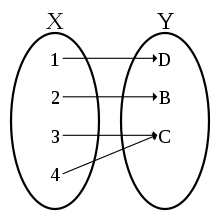
\includegraphics[width=0.25\textwidth]{surjective-function.png}}
    \caption{A surjective function from domain $X$ to codomain $Y$.}
\end{figure}
\begin{definition}
    \textbf{(Injective function).} Let $f$ be a function whose domain is a set $X$. The function $f$ is said to be \textbf{injective} (or \textbf{one-to-one}), provided that for all $a$ and $b$ in $X$, whenever $f\left( a \right) = f\left( b \right)$, then $a = b$. Symbolically,
    \begin{equation}
        \textrm{If } f:X\to Y\textrm{, then $f$ is injective if }\forall\ a, b\in X,\ f\left( a \right) = f\left( b \right) \implies a = b.
    \end{equation}
\end{definition}
\begin{figure}[htbp]
    \centering
    \begin{subfigure}{.25\textwidth}
        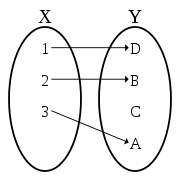
\includegraphics[width=\textwidth]{injective-nonsurjective-func.png}
        %\caption{An injective non-surjective function.}
    \end{subfigure}
    \hspace{1cm}
    \begin{subfigure}{.25\textwidth}
        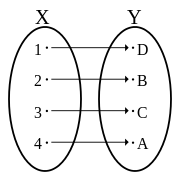
\includegraphics[width=\textwidth]{injective-surjective-func.png}
        %\caption{An injective surjective function.}
    \end{subfigure}
    %\centerline{\includegraphics[width=0.3\textwidth]{injective-function.png}}
    \caption{Injective non-surjective function (left) / Injective surjective function (right).}
\end{figure}

\begin{definition}
    \textbf{(Bijective function).} Let $f$ be a function from a set $X$ to a set $Y$. The function $f$ is said to be \textbf{bijective} if it's both surjective and injective. In other words, each element of one set is paired with exactly one element of the other set, and each element of the other set is paired with exactly one element of the first set.
\end{definition}

\begin{remark}
    If $X$ and $Y$ are finite sets, then the existence of a bijection means they have the same number of elements.
\end{remark}
\begin{figure}[htbp]
    \centerline{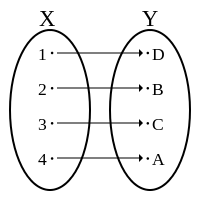
\includegraphics[width=0.25\textwidth]{bijective-func.png}}
    \caption{A bijective function, $f:X\to Y$.}
\end{figure}

A bijective function from the set $X$ to the set $Y$ has an \textbf{inverse function} from $Y$ to $X$.

%\subsubsection{Inverse functions}
\begin{definition}
    \textbf{(Inverse function).} Let $f$ be a function whose domain is the set $X$, and whose codomain is the set $Y$. Then, $f$ is \textbf{invertible} if there exists a function $g$ with domain $Y$ and image $X$, with the property
    \begin{equation}
        f\left( x \right) = y \iff g\left( y \right) = x
    \end{equation}
\end{definition}

If $f$ is invertible, then the function $g$ is unique, which means that there is exactly one function $g$ satisfying this property. That function $g$ is then called the \textbf{inverse} of $f$, usually denoted as $f^{-1}$.
\begin{proposition}
    If $f$ is an invertible function with domain $X$ and range $Y$, then
    \begin{equation}
        f^{-1}\left( f\left( x \right)  \right) = x,\quad \forall\ x\in X.
    \end{equation}
\end{proposition}
\begin{example}[Let $g:\R\to\R$ be a bijective function which $x\mapsto 2x + 1$. Calculate $g^{-1}:\R\to\R$.]
    In order to calculate the inverse of a bijective function we should write the function in terms of $y$ and then change $y$ for $x$.
    \begin{equation}
        2x + 1 = y \quad\iff\quad x = \frac{y - 1}{2} \quad\rightarrow\quad g^{-1} = y = \frac{x - 1}{2}
    \end{equation}
    \begin{align}
        g^{-1}:\R&\to\R \\ x&\mapsto \frac{x - 1}{2}
    \end{align}
\end{example}
